\documentclass[12pt]{article}
\usepackage{booktabs, multicol, graphicx}
\usepackage{setspace}
\setstretch{1.2}
\usepackage[a4paper]{geometry}
\geometry{hscale=0.7,vscale=0.75,centering}

\begin{document}

\section*{Supplementary material}


This supplementary material provides results on forecast performance of middle-level series defined by the natural hierarchy. For cluster hierarchies and two-level hierarchies where these middle-level series do not exist, we compute the middle-level forecasts using a bottom-up strategy. The average RMSSE based on different approaches for the tourism and mortality datasets are presented in Table~\ref{tab:P3_rmsse}. The MCB test results on middle-level series are shown in Figure~\ref{fig:mcb_middle}.\\



\begin{table}[!h]
\renewcommand\thetable{S.1}
    \centering
\caption{\label{tab:P3_rmsse}Performance of all approaches in terms of average RMSSE across all evaluation windows on both datasets. Column-wise minimum values are displayed in bold. ``Middle'' refers to middle-levels defined by the natural hierarchy. }
\vspace{0.1in}
\begin{tabular}{lcccccc}
\toprule
 Approach & \multicolumn{3}{c}{tourism} & \multicolumn{3}{c}{mortality} \\ 
 \cmidrule(lr){2-4} \cmidrule(lr){5-7}
 & Top & Middle & Bottom & Top & Middle & Bottom \\ \midrule
 Base & \textbf{0.869} & 0.732 & 0.694 & 0.761 & 0.744 & 0.753 \\
Two-level & 0.923 & 0.730 & 0.694 & 0.736 & 0.735 & 0.753 \\
Natural & 0.876 & \textbf{0.717} & 0.691 & 0.738 & 0.732 & 0.750 \\
Grouped & 0.831  & 0.721 & 0.706 & 0.798 & 0.783 & 0.750 \\
TS-EUC-ME & 0.900 & 0.727 & 0.693 & 0.728 & 0.735 & 0.753 \\
ER-EUC-ME & 0.918 & 0.727 & 0.693 & 0.741 & 0.740 & 0.753 \\
TSF-EUC-ME & 0.907 & 0.728 & 0.693 & 0.739 & 0.741 & 0.755 \\
ERF-EUC-ME & 0.909 & 0.729 & 0.694 & 0.733 & 0.738 & 0.753 \\
TS-EUC-HC & 0.874 & 0.719 & 0.692 & 0.740 & 0.730 & 0.754 \\
ER-EUC-HC & 0.890 & 0.719 & 0.691 & 0.746 & 0.732 & 0.751 \\
TSF-EUC-HC & 0.881 & 0.719 & 0.690 & 0.744 & 0.739 & 0.751 \\
TS-DTW-ME & 0.909 & 0.729 & 0.693 & \textbf{0.726} & 0.734 & 0.753 \\
TS-DTW-HC & 0.878 & 0.719 & 0.691 & 0.731 & 0.730 & 0.750 \\
ER-DTW-ME & 0.911 & 0.729 & 0.694 & 0.733 & 0.739 & 0.753 \\
ER-DTW-HC & 0.878 & 0.719 & 0.691 & 0.748 & 0.736 & 0.753 \\ 
Combination & 0.893 & 0.721 & \textbf{0.690} & 0.730 & \textbf{0.724} & \textbf{0.725} \\
\bottomrule\end{tabular}

\end{table}

\begin{figure}
\renewcommand\thefigure{S.1}
    \centering
    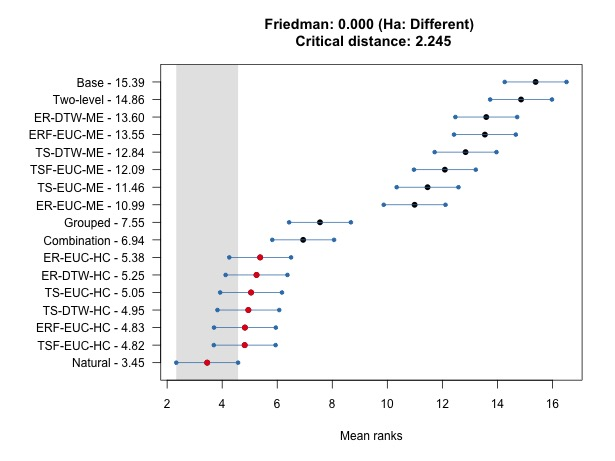
\includegraphics[width=0.5\textwidth]{../figures/FigureS1_tourism_mcb_combination_middle.jpg}
    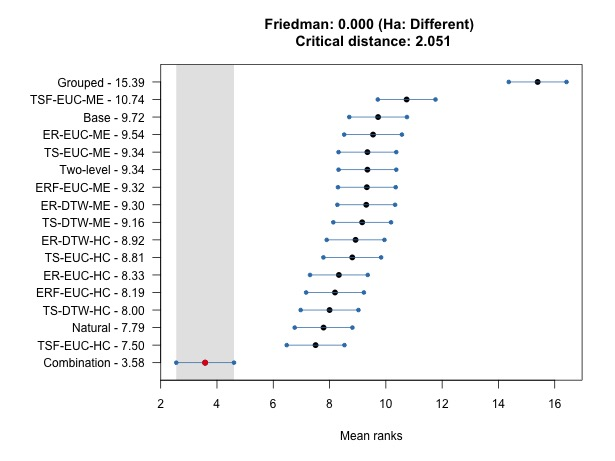
\includegraphics[width=0.5\textwidth]{../figures/Figure12_mortality_mcb_combination.jpg}
    \caption{\label{fig:mcb_middle}Average ranks and 95\% confidence intervals for all approaches on middle level of tourism dataset (left) and mortality dataset (right) based on MCB test.}
\end{figure}

\end{document}